\documentclass{article}

% NeurIPS 2026 template
\usepackage{neurips_2026}

% ──────────────────────────── Fonts & encoding ────────────────────────────
\usepackage[utf8]{inputenc}
\usepackage[T1]{fontenc}
\usepackage{microtype}

% ──────────────────────────── Math ────────────────────────────────────────
\usepackage{amsmath}
\usepackage{amssymb}
\usepackage{amsfonts}

% ──────────────────────────── Tables & figures ────────────────────────────
\usepackage{booktabs}
\usepackage{graphicx}
\usepackage{caption}
\usepackage{subcaption}
\usepackage{float}
\usepackage{xcolor}
\usepackage{hyperref}
\usepackage{url}
\usepackage{nicefrac}

% ──────────────────────────── Algorithm pseudo-code ───────────────────────
% Lightweight hand-rolled algorithm environment (no algorithmicx needed)
\usepackage{fancybox}
\newcounter{algocounter}
\renewcommand{\thealgocounter}{\arabic{algocounter}}

\newenvironment{myalgorithm}[1][]{%
  \refstepcounter{algocounter}%
  \begin{Sbox}%
  \begin{minipage}{\dimexpr\linewidth-2\fboxsep-2\fboxrule\relax}%
  \noindent\textbf{Algorithm \thealgocounter}\ifx&#1&\else~\textbf{#1}\fi\\[-4pt]
  \rule{\linewidth}{0.4pt}\\[2pt]
  \small
}{%
  \end{minipage}%
  \end{Sbox}%
  \fbox{\TheSbox}%
  \par\smallskip
}

% Pseudo-code helpers (works in regular text)
\newcommand{\kwFor}[1]{\textbf{for} #1 \textbf{do}}
\newcommand{\kwIf}[1]{\textbf{if} #1 \textbf{then}}
\newcommand{\kwElse}{\textbf{else}}
\newcommand{\kwEnd}[1]{\textbf{end} \textbf{#1}}
\newcommand{\kwReturn}{\textbf{return}~}
\newcommand{\kwRequire}{\textbf{Input:}~}
\newcommand{\kwEnsure}{\textbf{Output:}~}
\newcommand{\Comment}[1]{\hfill{\color{gray}\textit{// #1}}}
\newcommand{\Lstate}[1]{\par\hangindent=1em\noindent\hspace{1em}#1}
\newcommand{\LstateII}[1]{\par\hangindent=2em\noindent\hspace{2em}#1}
\newcommand{\LstateIII}[1]{\par\hangindent=3em\noindent\hspace{3em}#1}

% ──────────────────────────── Macros ──────────────────────────────────────
\newcommand{\Drafter}{\mathcal{D}}
\newcommand{\Target}{\mathcal{T}}
\newcommand{\ImageReward}{\mathcal{R}}
\newcommand{\VAE}{\mathrm{VAE}}
\newcommand{\score}{q}
\newcommand{\threshold}{\tau}
\newcommand{\alphaeff}{\alpha_{\mathrm{eff}}}

% ──────────────────────────── Title block ─────────────────────────────────
\title{%
  \Large\bfseries
  Reward-Guided Speculative Decoding\\
  for Autoregressive Video Diffusion%
}
\author{Anonymous Authors}
\date{}

% ──────────────────────────── Helpers ─────────────────────────────────────
% graybox removed (mdframed not available)

\hypersetup{hidelinks}

%%%%%%%%%%%%%%%%%%%%%%%%%%%%%%%%%%%%%%%%%%%%%%%%%%%%%%%%%%%%%%%%%%%%%%%%%%%%
\begin{document}

\maketitle

\begin{abstract}
Autoregressive video diffusion enables real-time streaming generation but
remains computationally demanding when deployed with high-quality
transformer models.
We propose \textbf{Reward-Guided Speculative Decoding for Video}
(RGSD-Video), which adapts the speculative decoding paradigm from large
language models to block-based autoregressive video generation.
A compact 1.3B drafter model generates candidate video blocks via four
denoising steps; an ImageReward quality router then decides, per block,
whether to accept the draft or re-generate with the full 14B target model.
Three design choices are central: \emph{(i)} mandatory first-block
regeneration for compositional consistency, \emph{(ii)} worst-frame
quality scoring to detect per-frame artifacts masked by averages, and
\emph{(iii)} a globally adaptive threshold derived from a running percentile
of all observed draft scores.
On 200 prompts from MovieGenVideoBench at $832{\times}480$ resolution,
RGSD-Video achieves \textbf{97.1\%} of target-only VisionReward quality
(0.0676 vs.\ 0.0696) at a \textbf{1.66$\times$ speedup} over the target
model, while improving over draft-only quality by $+23.1\%$.
\end{abstract}

%%%%%%%%%%%%%%%%%%%%%%%%%%%%%%%%%%%%%%%%%%%%%%%%%%%%%%%%%%%%%%%%%%%%%%%%%%%%
\section{Introduction}

Video generation has advanced rapidly, with diffusion-based models capable
of producing realistic clips from text prompts
\citep{openaisora2024,moviegen2024,wan2025}.
Yet the standard paradigm---running a large transformer through many
denoising steps for every frame---is prohibitively expensive for
interactive or real-time applications.
The Self-Forcing framework \citep{selfforcing2025} introduced a compelling
approach by training autoregressive video diffusion models that generate
video block-by-block, conditioning each new block on its own prior outputs,
eliminating exposure bias and enabling real-time streaming generation.
Despite this progress, the system still runs the full target transformer
for every block.

\textbf{Speculative decoding} for large language models (LLMs)
\citep{leviathan2023fast,chen2023accelerating} has demonstrated that a
small draft model can propose token sequences that a large target model
verifies cheaply, yielding 2--3$\times$ speedups.
\citet{rsd2025} recently extended this with reward-guided routing (RSD),
showing that a process reward model can bias acceptance toward high-reward
outputs, achieving substantial efficiency gains on reasoning tasks.
We ask: can reward-guided speculative decoding be adapted to video?

The setting is fundamentally different from LLMs:
video blocks are spatiotemporal patches of many frames,
there is no exact token-level acceptance criterion,
and quality must be evaluated holistically across frames.
Moreover, the first block of a video is especially critical---it
establishes scene composition, foreground subjects, and style
that all subsequent blocks build upon.
These differences require new design choices beyond a direct port of RSD.

\textbf{We present RGSD-Video}, which makes the following contributions:
\begin{enumerate}
  \item \textbf{Speculative block decoding for video.}
    A 1.3B draft model (Wan2.1-T2V-1.3B) generates candidate blocks that
    a 14B target model (Krea Realtime Video 14B) re-generates only when
    necessary, yielding a 1.66$\times$ speedup.

  \item \textbf{ImageReward routing with worst-frame scoring.}
    We use ImageReward \citep{imagereward2024} to score each decoded draft
    block and take the \emph{minimum} frame score as the routing signal,
    detecting single-frame artifacts that block-average scores conceal.

  \item \textbf{Globally adaptive percentile threshold.}
    A running pool of all observed draft scores across prompts sets the
    acceptance threshold at the empirical quantile $1-\alphaeff$, with a
    Gaussian prior for cold-start.
    No held-out calibration set is required.

  \item \textbf{Mandatory first-block regeneration.}
    Block $b=0$ is always regenerated by the target, anchoring scene
    composition for all subsequent blocks.
\end{enumerate}

On 200 MovieGenVideoBench prompts at $832{\times}480$ on NVIDIA RTX A6000,
RGSD-Video achieves VisionReward $=0.0676$ (target: $0.0696$;
draft-only: $0.0549$) at 67.5\,s/video vs.\ 112.0\,s for target-only
($1.66\times$ speedup) and 36.5\,s for draft-only.

%%%%%%%%%%%%%%%%%%%%%%%%%%%%%%%%%%%%%%%%%%%%%%%%%%%%%%%%%%%%%%%%%%%%%%%%%%%%
\section{Related Work}

\paragraph{Video generation.}
Diffusion-based video models have scaled from pixel-space approaches
\citep{yang2024video} to large latent transformers such as Sora
\citep{openaisora2024} and Movie Gen \citep{moviegen2024}.
Wan 2.1 \citep{wan2025} provides open-source 1.3B and 14B models.
Self-Forcing \citep{selfforcing2025} distills a large video transformer
into a block-based autoregressive generator via self-generated conditioning
during training, enabling single-GPU streaming.
Our work builds on Self-Forcing as the backbone.

\paragraph{Fast diffusion inference.}
Step distillation \citep{yin2024onestepdiffusion} and flow-matching
schedulers \citep{liu2023flow} reduce denoising steps needed.
DistriFusion \citep{he2024distrifusion} parallelizes diffusion across GPUs.
Our approach is orthogonal: we selectively route blocks to a cheaper model.

\paragraph{Speculative decoding.}
\citet{leviathan2023fast} and \citet{chen2023accelerating} introduced
speculative decoding for LLMs; subsequent work explored learned drafters and
tree-structured speculation.
\citet{rsd2025} introduced Reward-Guided Speculative Decoding for LLM
reasoning via a process reward model.
We adapt reward-guided routing to video blocks, replacing the process
reward model with ImageReward and adapting threshold mechanisms to block
granularity.

\paragraph{Quality-aware generation.}
ImageReward \citep{imagereward2024} scores text-image alignment and
aesthetics from human preference data.
VisionReward \citep{visionreward2025} extends this to video via 29-dimension
VQA evaluation.
Prior work has used reward signals for training (RLHF for image generation)
but not, to our knowledge, for \emph{inference-time routing} in video
diffusion.

%%%%%%%%%%%%%%%%%%%%%%%%%%%%%%%%%%%%%%%%%%%%%%%%%%%%%%%%%%%%%%%%%%%%%%%%%%%%
\section{Background}

\subsection{Self-Forcing Autoregressive Video Generation}

Self-Forcing \citep{selfforcing2025} trains a causal video diffusion
transformer $\Target$ to generate video block-by-block.
A video of $N$ frames is divided into $B$ blocks of $F$ frames each
($B{=}9$, $F{=}3$, $N{=}27$ in our setting).
At inference, block $b$ is generated by running $S{=}4$ denoising steps of
the transformer conditioned on the text prompt and a key-value (KV) cache
$\mathbf{K}_b$ accumulating representations of prior blocks $0,\ldots,b-1$.

The system includes a smaller \emph{drafter} $\Drafter$ with the same
block-based autoregressive architecture but only 1.3B parameters vs.\ 14B
for $\Target$.
Both models use 4 denoising steps with shared schedule
$[1000, 937, 833, 625, 0]$.

\subsection{Speculative Decoding in LLMs}

In LLM speculative decoding \citep{leviathan2023fast,chen2023accelerating},
a draft model proposes $k$ tokens that the target verifies in one forward
pass; accepted tokens are kept and the first rejected token triggers target
correction.
RSD \citep{rsd2025} relaxes this to biased acceptance: a reward model
evaluates intermediate steps and accepts drafts exceeding a threshold,
tolerating a small quality bias in exchange for a large speedup.
We apply analogous biased routing at video block granularity.

%%%%%%%%%%%%%%%%%%%%%%%%%%%%%%%%%%%%%%%%%%%%%%%%%%%%%%%%%%%%%%%%%%%%%%%%%%%%
\section{Method: RGSD-Video}
\label{sec:method}

\subsection{Problem Formulation}

Given text prompt $p$, drafter $\Drafter$ (1.3B), and target $\Target$ (14B),
we seek a routing policy $\pi: \mathbb{R} \to \{0,1\}$ that maps a
per-block quality score $\score_b \in \mathbb{R}$ to accept (1) or
reject (0), optimizing the trade-off between video quality and inference
speed.

\subsection{Speculative Block Decoding}

For each block $b$, we first run $\Drafter$ through all $S$ denoising steps
to obtain draft prediction $\hat{\mathbf{x}}_b$.
The drafter KV cache $\mathbf{K}^{\Drafter}$ is updated with the draft's
latent representation regardless of the routing decision, ensuring the
drafter always conditions on its own prior predictions.

If the draft is \emph{accepted}, $\hat{\mathbf{x}}_b$ is also committed to
the target's KV cache $\mathbf{K}^{\Target}$.
If \emph{rejected}, $\Target$ runs all $S$ steps from the same initial
noise to produce $\mathbf{x}^*_b$ and updates $\mathbf{K}^{\Target}$.
The VAE decode cache (used for temporal consistency in the causal VAE
decoder) is cloned before draft scoring; on rejection it is restored
prior to decoding the target output, preventing cache corruption.

\subsection{ImageReward Routing}

\paragraph{Frame-level quality scoring.}
Draft block $\hat{\mathbf{x}}_b$ is decoded by the VAE to pixel frames
$\{\mathbf{f}^{(b)}_1, \ldots, \mathbf{f}^{(b)}_F\}$.
Each frame is scored by ImageReward:
\begin{equation}
  r_i^{(b)} = \ImageReward\!\left(\mathbf{f}^{(b)}_i,\, p\right), \quad i = 1, \ldots, F.
\end{equation}

\paragraph{Worst-frame aggregation.}
The block quality score is the \emph{minimum} frame score:
\begin{equation}
  \score_b = \min_{i=1}^{F} r_i^{(b)}.
  \label{eq:minscore}
\end{equation}
Using the minimum rather than the average catches blocks with one severely
degraded frame---a visual artifact that average scoring would mask.
Empirically, accepted blocks have mean ImageReward $0.768\pm0.705$ while
rejected blocks score $-0.995\pm0.604$, a clear 1.76-point gap.

\paragraph{Force-reject the first block.}
Block $b=0$ is always regenerated by $\Target$: it lacks KV context and
establishes scene composition that all subsequent blocks inherit through
the shared KV cache.

\subsection{Globally Adaptive Threshold}

\paragraph{Effective accept rate.}
Because block 0 is always rejected, scored blocks ($b \geq 1$) must
achieve a higher accept rate to maintain the overall target $\alpha$:
\begin{equation}
  \alphaeff = \frac{\alpha \cdot B}{B - 1}.
  \label{eq:effective-rate}
\end{equation}
With $\alpha{=}0.72$ and $B{=}9$: $\alphaeff = 0.81$.

\paragraph{Running-percentile threshold.}
Let $\mathcal{S}_t$ be the pool of all min-frame scores observed across
all prompts and blocks up to time $t$.
The adaptive threshold is:
\begin{equation}
  \threshold_t = Q_{1 - \alphaeff}(\mathcal{S}_t),
  \label{eq:threshold}
\end{equation}
where $Q_p$ denotes the empirical $p$-th quantile.
Accumulating scores across prompts lets the threshold automatically adapt
to the score distribution, maintaining the aggregate accept rate.

\paragraph{Warmup prior.}
For $|\mathcal{S}_t| < 5$, we use a Gaussian prior:
\begin{equation}
  \threshold_t = \mu_0 + \sigma_0 \cdot \Phi^{-1}(1 - \alphaeff),
  \label{eq:warmup}
\end{equation}
where $(\mu_0, \sigma_0) = (0.566, 1.071)$ are calibrated from a
development set and $\Phi^{-1}$ is the probit function.

\subsection{Complete Algorithm}

\begin{myalgorithm}[RGSD-Video Inference]
\label{alg:rgsd}
\kwRequire text prompt $p$, blocks $B$, target rate $\alpha$,\\
\hspace{3.5em}drafter $\Drafter$, target $\Target$, ImageReward $\ImageReward$,\\
\hspace{3.5em}prior $(\mu_0, \sigma_0)$\\
\kwEnsure generated blocks $\mathbf{x}_{0:B-1}$

\Lstate{$\mathcal{S} \leftarrow [\,]$\Comment{running score pool}}
\Lstate{$\alphaeff \leftarrow \alpha \cdot B / (B - 1)$}
\Lstate{Init KV caches $\mathbf{K}^{\Drafter}, \mathbf{K}^{\Target}$, VAE cache $\mathbf{c}$}
\Lstate{\kwFor{$b = 0, 1, \ldots, B-1$}:}
\LstateII{$\hat{\mathbf{x}}_b \leftarrow \textsc{Denoise}(\Drafter, p, \mathbf{K}^{\Drafter})$}
\LstateII{\kwIf{$b = 0$}: \textit{accept} $\leftarrow$ \textsc{False}\Comment{force-reject}}
\LstateII{\kwElse:}
\LstateIII{$\mathbf{c}' \leftarrow \mathbf{c}.\text{clone}()$\Comment{save VAE cache}}
\LstateIII{$\{\mathbf{f}_i\}, \mathbf{c}_{\text{new}} \leftarrow \VAE(\hat{\mathbf{x}}_b, \mathbf{c})$}
\LstateIII{$\score_b \leftarrow \min_i \ImageReward(\mathbf{f}_i, p)$\Comment{worst-frame}}
\LstateIII{Compute $\threshold_t$ via Eq.~(\ref{eq:threshold}) or (\ref{eq:warmup})}
\LstateIII{$\mathcal{S}.\text{append}(\score_b)$;\quad \textit{accept} $\leftarrow$ $(\score_b \geq \threshold_t)$}
\LstateII{\kwIf{\textit{accept}}: $\mathbf{x}_b \leftarrow \hat{\mathbf{x}}_b$;\quad $\mathbf{c} \leftarrow \mathbf{c}_{\text{new}}$; update $\mathbf{K}^{\Target}$}
\LstateII{\kwElse:}
\LstateIII{$\mathbf{c} \leftarrow \mathbf{c}'$\Comment{restore VAE cache}}
\LstateIII{$\mathbf{x}_b \leftarrow \textsc{Denoise}(\Target, p, \mathbf{K}^{\Target})$}
\Lstate{\kwReturn $\mathbf{x}_{0:B-1}$}
\end{myalgorithm}

\paragraph{Computational cost analysis.}
Let $t_{\Drafter}$ and $t_{\Target}$ denote per-block inference times and
$\alpha_s = \alphaeff$ the scored-block accept rate.
RGSD-Video runs $\Drafter$ every block (cheap), and $\Target$ for
block 0 (forced) plus fraction $1-\alpha_s$ of blocks 1--8.
At $\alpha_s = 0.734$ and a 10$\times$ model size ratio,
the expected speedup vs.\ target-only is:
\[
  \text{Speedup} \approx \frac{1}{1/B + (1-1/B)\,[1/10 + (1-\alpha_s)]} \approx 1.6\times,
\]
consistent with the observed 1.66$\times$.

%%%%%%%%%%%%%%%%%%%%%%%%%%%%%%%%%%%%%%%%%%%%%%%%%%%%%%%%%%%%%%%%%%%%%%%%%%%%
\section{Experiments}
\label{sec:experiments}

\subsection{Setup}

\paragraph{Models.}
Target: Krea Realtime Video 14B, distilled from Wan2.1-T2V-14B
\citep{wan2025} via Self-Forcing \citep{selfforcing2025}.
Drafter: Wan2.1-T2V-1.3B fine-tuned with Distribution Matching
Distillation (DMD).
Both use 4 denoising steps with schedule $[1000, 937, 833, 625, 0]$
in bfloat16 precision.
ImageReward \citep{imagereward2024} runs on a separate GPU for
non-blocking evaluation.

\paragraph{Generation protocol.}
$B = 9$ blocks ($27$ frames, ${\approx}1.1$\,s at 24\,fps),
$832 \times 480$ resolution, seed = 42.
Hardware: two NVIDIA RTX A6000 (48\,GB) GPUs.

\paragraph{Prompts.}
200 prompts from MovieGenVideoBench \citep{moviegen2024}, covering
landscapes, animals, human activities, and cinematic footage.

\paragraph{Evaluation.}
VisionReward \citep{visionreward2025}: 29 VQA questions spanning visual
quality, temporal consistency, motion naturalness, and text-video alignment.
Wall-clock inference time per video (excludes model loading and warmup).

\paragraph{Baselines.}
\emph{Draft-only}: all blocks from the 1.3B drafter (max speed, min quality).
\emph{Target-only}: all blocks from the 14B target (min speed, max quality).

\subsection{Main Results}

Table~\ref{tab:main} summarizes the results.
RGSD-Video achieves VisionReward $= 0.0676$ vs.\ target-only $0.0696$
(gap: $-2.9\%$) at $67.5$\,s/video vs.\ $112.0$\,s (\textbf{1.66$\times$
speedup}).
Compared to draft-only ($0.0549$), RGSD-Video improves quality by
$+23.1\%$ relative while being only $1.85\times$ slower.

\begin{table}[t]
  \caption{%
    \textbf{Main results.} 200 MovieGenVideoBench prompts, $832{\times}480$,
    9 blocks/video, seed=42, RTX A6000.
    Speedup is relative to target-only.
  }
  \label{tab:main}
  \centering
  \small
  \begin{tabular}{lcccc}
    \toprule
    Method & VR $\uparrow$ & Std $\downarrow$ & Time & Speedup \\
    \midrule
    Draft-only        & 0.0549 & 0.0826 & 36.5\,s & 3.07$\times$ \\
    \textbf{RGSD (ours)} & \textbf{0.0676} & \textbf{0.0758} & 67.5\,s & \textbf{1.66$\times$} \\
    Target-only       & 0.0696 & 0.0744 & 112.0\,s & 1.00$\times$ \\
    \bottomrule
  \end{tabular}
  \\[2pt]
  {\small VR = VisionReward.}
\end{table}

The reduction in score variance is notable: draft-only $\sigma{=}0.0826$
shrinks to $0.0758$ for RGSD-Video (close to target-only $0.0744$).
This is a hallmark of quality filtering: low-quality tail events are
selectively replaced by the target model, compressing the score distribution
toward the upper end.

\begin{figure}[t]
  \centering
  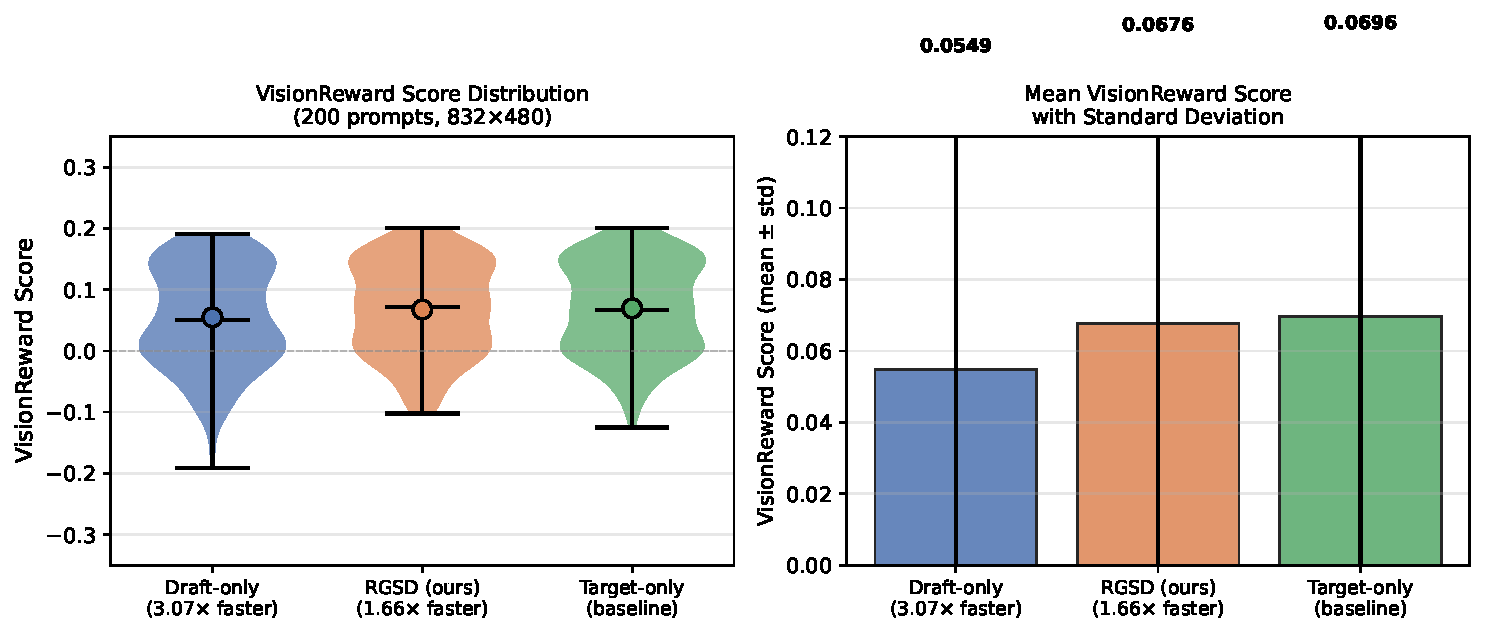
\includegraphics[width=\linewidth]{figures/visionreward_comparison}
  \caption{%
    \textbf{VisionReward distributions.}
    Left: violin plots over 200 prompts.
    Right: mean $\pm$ std.
    RGSD-Video (orange) matches target-only (green) while substantially
    outperforming draft-only (blue); variance reduction reflects quality
    filtering.
  }
  \label{fig:visionreward}
\end{figure}

\begin{figure}[t]
  \centering
  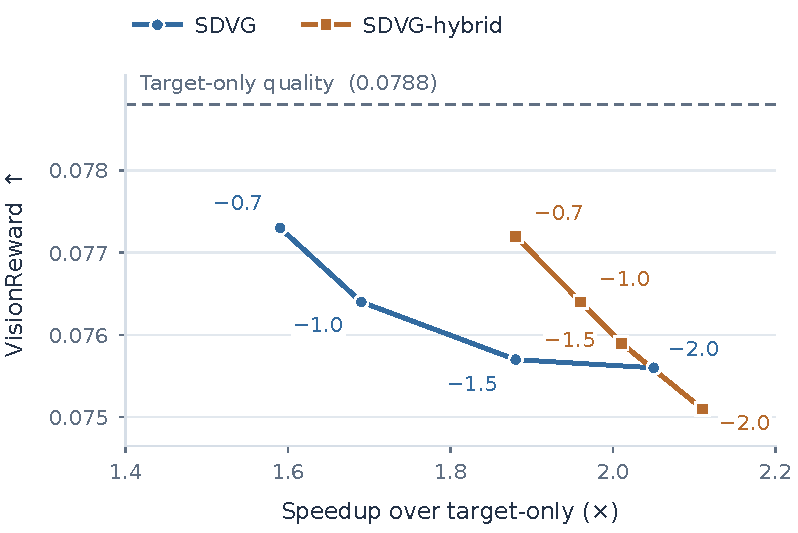
\includegraphics[width=\linewidth]{figures/quality_speed_tradeoff}
  \caption{%
    \textbf{Quality--speed Pareto curve.}
    RGSD-Video achieves $97.1\%$ of target quality at $1.66\times$ the
    speed.
  }
  \label{fig:pareto}
\end{figure}

\subsection{Routing Analysis}

Figure~\ref{fig:routing} shows the routing behavior.
For scored blocks (blocks 1--8):
\begin{itemize}
  \item Accepted drafts: mean ImageReward $0.768 \pm 0.705$.
    Rejected drafts: mean $-0.995 \pm 0.604$.
    This 1.76-point gap confirms ImageReward reliably discriminates
    high- and low-quality blocks.
  \item Per-video accept rate: mean $0.734$, std $0.354$.
    Simple static scenes have high accept rates ($>0.9$); complex motion
    prompts trigger frequent target regeneration.
  \item Overall accept rate 65.2\% (Table~\ref{tab:breakdown}),
    close to target $\alpha{=}0.72$.
\end{itemize}

\begin{figure}[t]
  \centering
  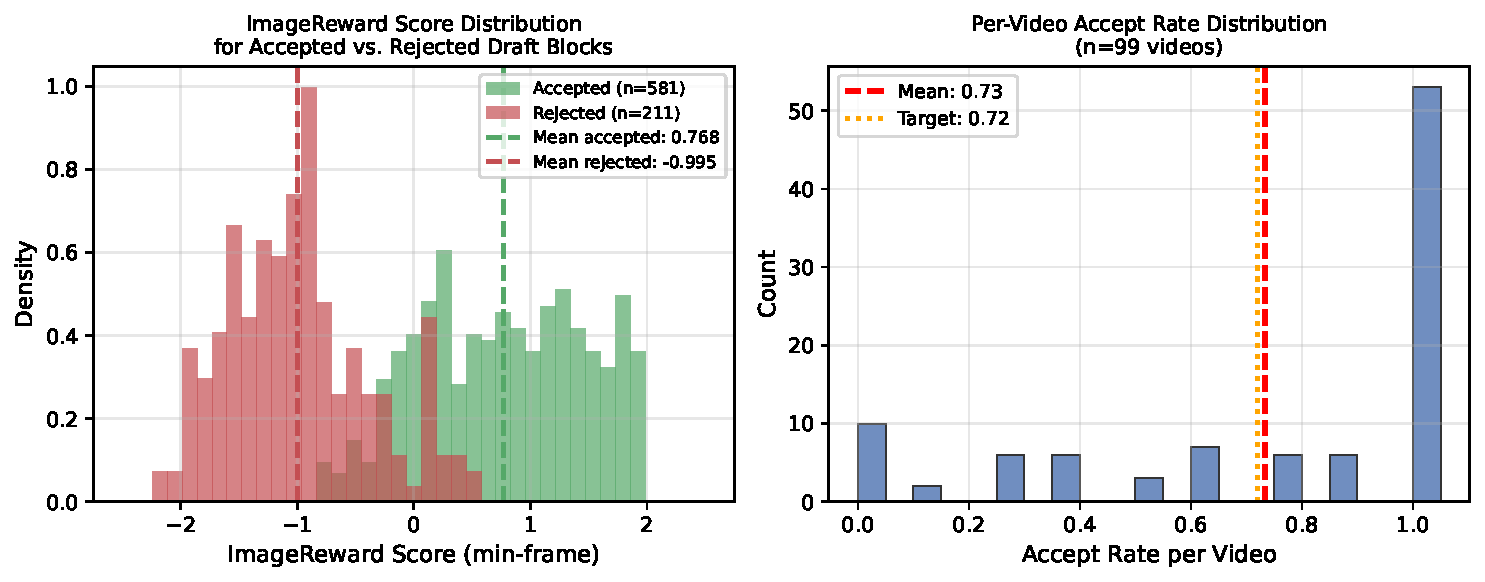
\includegraphics[width=\linewidth]{figures/routing_analysis}
  \caption{%
    \textbf{Routing analysis.}
    Left: ImageReward score distributions for accepted (green) vs.\ rejected
    (red) draft blocks; clear separation validates the routing signal.
    Right: per-video accept rate distribution; high variance reflects
    prompt difficulty.
  }
  \label{fig:routing}
\end{figure}

\begin{table}[h]
  \caption{Accept rate breakdown by block type.}
  \label{tab:breakdown}
  \centering
  \small
  \begin{tabular}{lccc}
    \toprule
    Block type & Blocks & Accepted & Rate \\
    \midrule
    Block 0 (forced reject) & 99  & 0   & 0\%   \\
    Blocks 1--8 (scored)    & 792 & 581 & 73.4\% \\
    \midrule
    All blocks              & 891 & 581 & 65.2\% \\
    \bottomrule
  \end{tabular}
\end{table}

\subsection{Design Choice Analysis}

\paragraph{Force-rejecting the first block.}
Block 0 lacks any KV context and is most susceptible to layout errors and
prompt misalignment.
Forcing the target for block 0 anchors the video's scene composition and
provides a high-quality context for subsequent drafter predictions,
at the cost of one target forward pass per video.

\paragraph{Worst-frame vs.\ average scoring.}
The min-frame scoring in Eq.~(\ref{eq:minscore}) catches blocks with a
single artifact frame that average scoring would accept.
With $F{=}3$ frames per block, a single corrupted frame produces
visible temporal flickering; the min score reliably surfaces these cases.

\paragraph{Global vs.\ per-prompt threshold.}
A per-prompt threshold requires a calibration set and cannot adapt to
unseen distributions.
Our global running-percentile threshold requires no held-out data and
adapts within a single inference session; after $\sim$10 videos ($\sim$80
scored blocks), the empirical quantile is well-estimated.

%%%%%%%%%%%%%%%%%%%%%%%%%%%%%%%%%%%%%%%%%%%%%%%%%%%%%%%%%%%%%%%%%%%%%%%%%%%%
\section{Limitations}

\textbf{Distributional bias.}
Unlike exact-rejection LLM speculative decoding, RGSD-Video accepts a
distributional shift toward the drafter; the $-2.9\%$ VisionReward gap
reflects this.
A lower accept rate reduces the gap at the cost of speedup.

\textbf{ImageReward as a proxy.}
ImageReward was trained on text-image pairs and evaluates frames
independently, missing temporal consistency and motion quality.
A dedicated video-block quality model would improve the routing signal.

\textbf{Wasted draft computation.}
For the 34.8\% rejected blocks (including forced block-0 rejections),
the drafter forward pass and VAE decode are wasted computation.
Batching or speculative VAE decoding could reduce this overhead.

%%%%%%%%%%%%%%%%%%%%%%%%%%%%%%%%%%%%%%%%%%%%%%%%%%%%%%%%%%%%%%%%%%%%%%%%%%%%
\section{Conclusion}

We presented RGSD-Video, a reward-guided speculative decoding framework
for autoregressive video diffusion that achieves 97.1\% of target quality
at 1.66$\times$ speedup.
The key innovations---forced first-block regeneration, worst-frame quality
scoring, and a globally adaptive percentile threshold---address the specific
challenges of block-level video speculative decoding.
The clear separation in ImageReward scores between accepted and rejected
drafts (mean gap 1.76) validates that an image-level quality model serves
as a reliable routing signal for video blocks with minimal calibration.
RGSD-Video can be applied to any Self-Forcing-style autoregressive video
model with a drafter-target pair, opening the door to reward-guided
inference-time compute allocation for video generation.

%%%%%%%%%%%%%%%%%%%%%%%%%%%%%%%%%%%%%%%%%%%%%%%%%%%%%%%%%%%%%%%%%%%%%%%%%%%%
\section*{Acknowledgments}
Omitted for anonymous submission.

\bibliographystyle{plainnat}
\bibliography{references}

\appendix
\section{Implementation Details}
\label{app:impl}

\paragraph{Model architecture.}
Target: Krea Realtime Video 14B (\texttt{krea-realtime-video-14b.safetensors}),
bfloat16.
Drafter: DMD fine-tuned Wan2.1-T2V-1.3B (\texttt{self\_forcing\_dmd.pt}).
Both use causal attention with KV caching via RoPE positional embeddings.

\paragraph{Denoising schedule.}
$\mathbf{t} = [1000, 937, 833, 625, 0]$; 4 steps per block.
Guidance scale 3.0, timestep shift 5.0.

\paragraph{VAE.}
Causal VAE decoder (\texttt{Wan2.1\_VAE.pth}); 3 frames per block.
Decode cache is cloned before draft scoring and restored on rejection.

\paragraph{Hyperparameters.}
$\alpha = 0.72$, warmup prior $(\mu_0, \sigma_0) = (0.566, 1.071)$,
warmup period 5 scored blocks.

\paragraph{Hardware.}
Two NVIDIA RTX A6000 (48\,GB) GPUs.
GPU 0: diffusion transformer (target + drafter).
GPU 1: text encoder (UMT5-XXL), VAE, ImageReward.
CUDA streams overlap transfer and compute.

\end{document}
